\chapter{Design}

\TODO{INTRO}


\section{System Architecture}

\TODO{High-Level description and block diagram}

\begin{figure}[!ht]
		\centering
		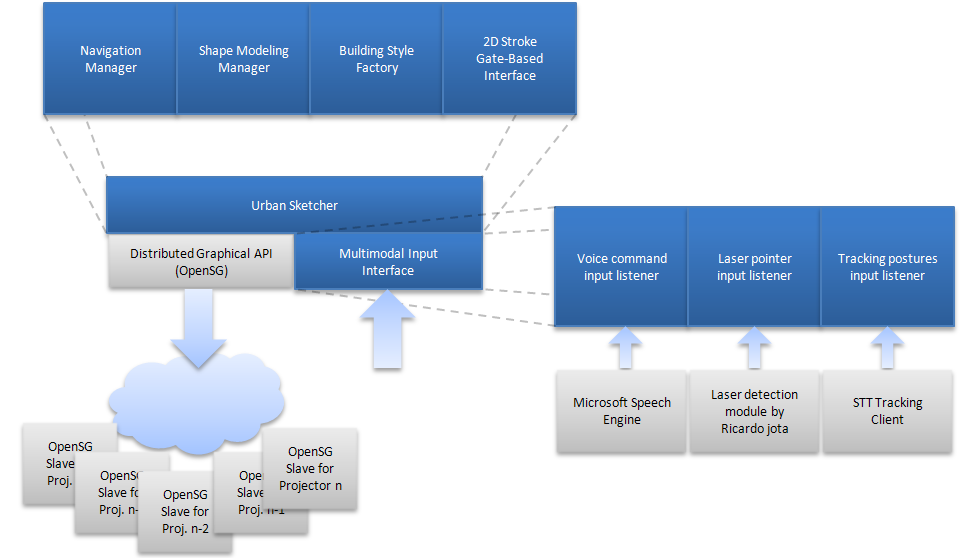
\includegraphics[width=17cm]{gfx/charts/block-diagram.png}
		\caption{Urban Sketcher Architecture Diagram}
		\label{fig:block-diagram}
\end{figure}

\TODO{REMOVE 'ricardo jota'; add mouse input; add broadcast and remove input arrow}

Urban Sketcher has as its core the following items\footnote{Blue items denote work done by the author.}:
\begin{itemize}
	\item The \textbf{Navigation Manager} is
		responsible for assembling navigation data from
		both voice+tracking input and gate events which trigger navigation changes,
		supporting several navigation modes;
	
	\item The \textbf{Shape Modeling Manager} is
		responsible for representing a 3D editable shape
		along with its geometry information, range of operations and a
		Memento Pattern for supporting undo operations;
	
	\item The \textbf{Building Style Factory} is
		responsible for parsing building style definitions
		and converting blueprints and height to actual building instances;
	
	\item The \textbf{2D Stroke-Based Interface} is 
		a set of interface widgets and their controllers,
		supporting option gates, ring menus and stroke-based operation handling.
	
\end{itemize}

Urban Sketcher gets input from several media:
laser pointers, the server machine's mouse and optionally voice commands and tracking postures.
The system can render to any number of slave machines.
An XML configuration allows parameterizing the range of machine and topology of the rendering slaves,
allowing the own machine to work as slave, a set of remote machines or both.


\section{Stroke-Based Input Interface}

This section details the concepts used in the creation of the interface for the system.

\subsection{Strokes}

A stroke is the result of continuous input from one laser pointer, from the time the laser
light button is pressed until it is released. 

By using the laser detection module, the system gets a stream of laser readings which
come sequentially tagged, that is, the module identifies with reasonable success when different strokes
occur simultaneously, returning both readings tagged with different stroke IDs.
Even so, the module can't infer whether different strokes came from the same source laser pointer.

This limitation sets an important assumption in our system -- one can not know whether 2 strokes came
from the same user, therefore operations must take place during at most the stroke period.

Strokes can also be emulated by using a mouse and pressing
the button as if it were a laser pointer.


\TODO{apply-to-scene}


\subsection{Gates}

The most common activation action in current Graphical User Interface (GUI) computer interactions work
by displaying a button on the screen and the user activating it by pressing the pointer device button.
Given that users will rely on laser pointers to interact with the GUI, a limitation derives from
using them instead of mice or track balls -- while a user isn't pressing the laser light button,
neither the system nor the user himself can know accurately where on the screen the laser is pointing to.
In order for the user to see the laser projection on the screen he must be pressing the button.
This necessity \TODO{urges} for a different GUI solution.

Based on prior research by \cite{CROSSY}, the gate concept was implemented with slight changes.

A gate is an imaginary two dimensional line on the screen, bound by two visible extremes.
To activate it one must draw a stroke which crosses the line, as if scoring a goal.

Gates can have a text label or a suggestive image to symbolize the action they perform.
It was decided not to mix both representations -- if the gate is illustrated, a tooltip can be invoked
by approaching the gate's area of influence without crossing it, so the action can be avoided.

\TODO{IMAGE ACTIVATION GATE}


\subsection{Menus}

The menus in this system are ring-shaped, with the options (gates) distributed on top of the ring.
Menus aren't totally opaque so the main viewport remains visible.
Menus 




\subsection{Strokes Gestures}

invoke main menu
select face
select edge


\section{Multimodal Input Interface}

\subsection{Arm Posing Flight Mode}


\section{Content Creation Concepts}

\subsection{Building Styles}

\subsection{Building Styles}